%
% linespoints.tex
%
\renewcommand{\thisname}{Chart::LinesPoints}
\section{\thisname}
\name{\thisname}
\file{LinesPoints.pm}
\requires{Chart::Base, GD, Carp, FileHandle}
\begin{Description}
The class \thisclass creates a lines chart where additionally the
individual data points are marked with a symbol. (If you want just
lines without additional symbols, check \class{Chart::Lines} on page
\pageref{Chart::Lines}. If you want just symbols for the data points but
no lines, check \class{Chart::Points} on page \pageref{Chart::Points}.)
\thisclass is a subclass of \class{Chart::Base}.
\end{Description}

\example
\begin{figure}[ht]
  \begin{center}
    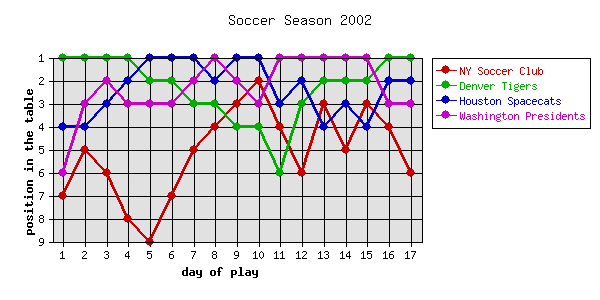
\includegraphics[scale=0.6]{d_linesp2.png}
  \end{center}
  \caption{Linespoints chart}
  \label{fig:d_linesp2}
\end{figure}
\begin{verbatim}
use Chart::LinesPoints;
use strict;

my (@data1, @data2, @data4, @data3, @labels, %hash, $g);

@labels = qw(1 2 3 4 5 6 7 8 9 10 11 12 13 14 15 16 17);
@data1  = qw (-7 -5 -6 -8 -9 -7 -5 -4 -3 -2 -4 -6 -3 -5 -3 -4 -6);
@data2  = qw (-1 -1 -1 -1 -2 -2 -3 -3 -4 -4 -6 -3 -2 -2 -2 -1 -1);
@data3  = qw (-4 -4 -3 -2 -1 -1 -1 -2 -1 -1 -3 -2 -4 -3 -4 -2 -2);
@data4  = qw (-6 -3 -2 -3 -3 -3 -2 -1 -2 -3 -1 -1 -1 -1 -1 -3 -3);

$g = Chart::LinesPoints->new(600,300);
$g->add_dataset(@labels);
$g->add_dataset(@data1);
$g->add_dataset(@data2);
$g->add_dataset(@data3);
$g->add_dataset(@data4);

%hash = ('integer_ticks_only' => 'true',
         'title'         => 'Soccer Season 2002\n ',
         'legend_labels' => ['NY Soccer Club', 'Denver Tigers',
                             'Houston Spacecats',
                             'Washington Presidents'],
         'y_label'       => 'position in the table',
         'x_label'       => 'day of play',
         'grid_lines'    => 'true',
         'f_y_tick'      => \&formatter,
        );

$g->set( %hash);

$g->png("d_linesp2.png");

# Just a trick to have the y scale start at the biggest point:
# Initialise with negative values, remove the minus sign!
sub formatter {
  my $label = shift;
  $label    = substr($label, 1);
  return $label;
}

\end{verbatim}

\constructorblurb{\thisname}

\begin{AttrDecl}{brush\_size}
Sets the width of the lines in pixels. Default is 6.
\end{AttrDecl}

\begin{AttrDecl}{brushStyle}
Define the share of the points. The share may be specified to each dataset.\\
The possible shapes of the 'points' are
\begin{itemize}
\item FilledCircle (default),
\item circle,
\item donut,
\item OpenCircle,
\item triangle,
\item upsidedownTriangle,
\item square,
\item hollowSquare,
\item OpenRectangle,
\item fatPlus,
\item Star,
\item OpenStar,
\item FilledDiamond, 
\item OpenDiamond
\end{itemize} 
To apply a different brush style to different data sets the following
example of code can be used:
\begin{verbatim}
$g->set(brushStyles => { dataset0 => 'fatPlus', dataset1 => 'hollowSquare' });
\end{verbatim}
\end{AttrDecl}


\begin{AttrDecl}{pt\_size}
Sets the radius of the points in pixels. Default is 18.
\end{AttrDecl}

\begin{AttrDecl}{sort}
Sorts the data in ascending order if set to \literal{true}. Should be
set if the input data is not sorted. Defaults to \literal{false}.
\end{AttrDecl}

\begin{AttrDecl}{stepline}
The points are connected by a stepping function,instead of by a direct
line if set to \literal{true}. Defaults to \literal{false}.
\end{AttrDecl}

\begin{AttrDecl}{stepline\_mode}
Determines whether to plot each stepping line at the level of the
start of the interval (if set to \literal{begin}) or at its end if set
to \literal{end}. Defaults to \literal{begin}.
\end{AttrDecl}

\attrdecl{xlabels}
\begin{AttrDecl}{xrange}
This pair of options allows arbitrary positioning of $x$ axis labels.
The two options must either both be specified or both be omitted.
\attruse{xlabels} is a reference to 2-element array. The first of the
elements is a nested (reference to an) array of strings that are the
labels. The second element is a nested (reference to an) array of
numbers that are the $x$ values at which the labels should be placed.
\attruse{xrange} is a 2-element array specifying the minimum and maximum
$x$ values on the axis. \Eg,
\begin{verbatim}
@labels = (['Jan', 'Feb', 'Mar'],
           [10,    40,    70   ]);
$chart->set(xlabels => \bs @labels,
            xrange  => [0, 100]
           );
\end{verbatim}
\end{AttrDecl}

\begin{AttrDecl}{xy\_plot}
Forces \thisclass to plot a $x$--$y$ graph if set to \literal{true}, \ie, to
treat the $x$ axis as numeric. Very useful for plots of mathematical
functions. Defaults to \literal{false}.
\end{AttrDecl}

\begin{AttrDecl}{y\_axes}
Tells \thisclass where to place the $y$ axis. Valid
values are \literal{left}, \literal{right} and \literal{both}. Defaults
to \literal{left}.
\end{AttrDecl}

